% Options for packages loaded elsewhere
\PassOptionsToPackage{unicode}{hyperref}
\PassOptionsToPackage{hyphens}{url}
\documentclass[
]{article}
\usepackage{xcolor}
\usepackage{amsmath,amssymb}
\setcounter{secnumdepth}{-\maxdimen} % remove section numbering
\usepackage{iftex}
\ifPDFTeX
  \usepackage[T1]{fontenc}
  \usepackage[utf8]{inputenc}
  \usepackage{textcomp} % provide euro and other symbols
\else % if luatex or xetex
  \usepackage{unicode-math} % this also loads fontspec
  \defaultfontfeatures{Scale=MatchLowercase}
  \defaultfontfeatures[\rmfamily]{Ligatures=TeX,Scale=1}
\fi
\usepackage{lmodern}
\ifPDFTeX\else
  % xetex/luatex font selection
\fi
% Use upquote if available, for straight quotes in verbatim environments
\IfFileExists{upquote.sty}{\usepackage{upquote}}{}
\IfFileExists{microtype.sty}{% use microtype if available
  \usepackage[]{microtype}
  \UseMicrotypeSet[protrusion]{basicmath} % disable protrusion for tt fonts
}{}
\makeatletter
\@ifundefined{KOMAClassName}{% if non-KOMA class
  \IfFileExists{parskip.sty}{%
    \usepackage{parskip}
  }{% else
    \setlength{\parindent}{0pt}
    \setlength{\parskip}{6pt plus 2pt minus 1pt}}
}{% if KOMA class
  \KOMAoptions{parskip=half}}
\makeatother
\usepackage{longtable,booktabs,array}
\newcounter{none} % for unnumbered tables
\usepackage{calc} % for calculating minipage widths
% Correct order of tables after \paragraph or \subparagraph
\usepackage{etoolbox}
\makeatletter
\patchcmd\longtable{\par}{\if@noskipsec\mbox{}\fi\par}{}{}
\makeatother
% Allow footnotes in longtable head/foot
\IfFileExists{footnotehyper.sty}{\usepackage{footnotehyper}}{\usepackage{footnote}}
\makesavenoteenv{longtable}
\usepackage{graphicx}
\makeatletter
\newsavebox\pandoc@box
\newcommand*\pandocbounded[1]{% scales image to fit in text height/width
  \sbox\pandoc@box{#1}%
  \Gscale@div\@tempa{\textheight}{\dimexpr\ht\pandoc@box+\dp\pandoc@box\relax}%
  \Gscale@div\@tempb{\linewidth}{\wd\pandoc@box}%
  \ifdim\@tempb\p@<\@tempa\p@\let\@tempa\@tempb\fi% select the smaller of both
  \ifdim\@tempa\p@<\p@\scalebox{\@tempa}{\usebox\pandoc@box}%
  \else\usebox{\pandoc@box}%
  \fi%
}
% Set default figure placement to htbp
\def\fps@figure{htbp}
\makeatother
\setlength{\emergencystretch}{3em} % prevent overfull lines
\providecommand{\tightlist}{%
  \setlength{\itemsep}{0pt}\setlength{\parskip}{0pt}}
\usepackage{bookmark}
\IfFileExists{xurl.sty}{\usepackage{xurl}}{} % add URL line breaks if available
\urlstyle{same}
\hypersetup{
  hidelinks,
  pdfcreator={LaTeX via pandoc}}

\author{}
\date{}

\begin{document}

\section{Capacity Scaling of Encoding-Through-Loading: Application
vs.~Cloze Asymmetry Across Three Orders of
Magnitude}\label{capacity-scaling-of-encoding-through-loading-application-vs.-cloze-asymmetry-across-three-orders-of-magnitude}

\textbf{Author:} Tomas Pødenphant Lund

\textbf{Affiliation:} Independent Research, Aarhus

\textbf{Correspondence:} tomas.lund@frictiontheory.org

\textbf{Web:} https://frictiontheory.org

\textbf{Target:} PNAS Perspective / Journal of Memory and Language /
Trends in Cognitive Sciences

\textbf{Acknowledgments:} Extensive discussion, literature search,
empirical analysis, and manuscript structuring were conducted in
collaboration with Claude (Anthropic, 2025--2026). The theoretical
claims, interpretations, and predictions are those of the author.

\textbf{Data and code availability:} Per-token logprob datasets,
analysis scripts, and figures are released at
\url{https://github.com/tplund/friction-theory-p2-capacity-scaling}
under CC BY 4.0.

\begin{center}\rule{0.5\linewidth}{0.5pt}\end{center}

\subsection{0. Abstract}\label{abstract}

Large language models solve two differentiable task types on the same
underlying knowledge base. \textbf{Cloze retrieval} --- recovering a
fact as presented --- saturates early: most models reach
\textasciitilde90\% accuracy by 8B parameters. \textbf{Application} ---
chaining multiple facts into a derivation --- scales monotonically
across three orders of magnitude, from 2\% at 0.5B to 85\% at 70B. We
document this asymmetry on a \textbf{single invented knowledge domain
(``Zorbetik'')} designed specifically to eliminate pretraining-prior
confounds, across nine models spanning 0.5B to 671B parameters, using
frontloaded in-context learning to expose encoding-to-retrieval dynamics
without weight updates. Generalisation to natural knowledge domains is a
direct next-step empirical extension of the methodology established
here.

Three findings follow. \textbf{Finding 1}: Application scales
monotonically with capacity (Spearman ρ = +1.000 on the Qwen2.5
sub-ladder, n=5, p = 0.0083 one-tailed / 0.0167 two-tailed; cross-family
panel ρ = +0.92, n=9, p = 0.0005 two-tailed; slope +40.8 percentage
points per decade). Cloze does not. \textbf{Finding 2}: The bottleneck
migrates with capacity --- at 0.5B, retrieval fails; at 14B, retrieval
is saturated and 36\% of questions show a ``retrieval succeeds,
derivation fails'' pattern. \textbf{Finding 3}: Mixture-of-Experts (MoE)
models scale on \textbf{active} parameters, not total. A 235B MoE with
22B active parameters behaves on application tasks like a 22B dense
model (active-parameter projection within 3pp of actual; total-parameter
projection off by 33pp).

We also advance a methodological claim: \textbf{frontloaded in-context
learning (ICL)} --- presenting all training facts in the prompt followed
by one question, with per-token logprobs captured on the answer ---
operationally substitutes for fine-tuning in encoding-to-retrieval
studies. It is fast (\textasciitilde5 seconds per inference vs.~hours
for FT), cheap (cents vs.~dollars), unified across model families, and
produces dense friction data (six statistics per inference). Caveats:
ICL is bounded by the context window and is ephemeral to each prompt, so
FT remains necessary for large knowledge bases, persistence studies, and
route-overwrite experiments.

\textbf{Implications.} Capacity is single-axis but loads task types
differentially. Cloze is indexing-bound; application is
composition-bound. The three-dimensional friction framework (magnitude,
distribution, rhythm) from Paper 1 decomposes the C-axis into
corresponding operational handles. Paper 4 systematically tests these
handles across classical learning phenomena.

\begin{center}\rule{0.5\linewidth}{0.5pt}\end{center}

\subsection{1. Introduction}\label{introduction}

Paper 1 (Lund 2026b) introduced \textbf{Friction Theory (FT)} as a
substrate-universal framework for probabilistic computation under
bounded resources, with Behavioural Friction Theory (BFT; Lund 2026a) as
its biological instantiation (BFT ⊂ FT). The framework predicted three
dimensions of friction (magnitude, distribution, rhythm) and identified
capacity (C) as the primary axis determining how much information can be
held and manipulated simultaneously. This paper tests the C-dimension
prediction on LLM substrate --- an FT-level test, not a BFT-level test,
because LLMs lack the biological fields that distinguish BFT from FT.

This paper tests the C-dimension's implication for
\emph{encoding-through-loading} --- the hypothesis (Paper 1 §6.4) that
learning is a direct consequence of route-competition under load, not a
separate cognitive module. Specifically, we examine how the same
underlying knowledge manifests differently through two distinct task
types --- cloze retrieval vs.~derivation-requiring application --- as
capacity is varied across three orders of magnitude.

Our central methodological move is the use of an \textbf{invented
knowledge domain} (``Zorbetik''). This eliminates pretraining priors as
a confound. When a model is presented with 47 facts about fictive
chemical processes and queried about properties of a fictive substance,
it cannot draw on prior exposure. What is measured is the substrate's
ability to integrate and use the just-presented information.

We measure three things simultaneously in a single prompt call: (a)
accuracy on cloze vs.~application, (b) per-token CR signal on the
answer, and (c) first-5-tokens friction as a proxy for how cleanly the
context integrated into the substrate's active state.

This paper focuses on the capacity axis. Paper 4 (Lund 2026e) tests
encoding-structure (how the same information is organized) × capacity
interaction --- a series of findings originally planned for this paper
but moved to keep scope focused.

\textbf{Structure.} §2 reports the empirical capacity-scaling results on
the Zorbetik domain, including the application/cloze asymmetry, the
bottleneck-migration finding, and the MoE active-vs-total parameter
analysis. §3 develops the frontloaded-ICL methodology as a substitute
for fine-tuning. §4 notes content moved to Paper 4. §5 discusses
implications for the C-dimension framework. §6 concludes.

\begin{center}\rule{0.5\linewidth}{0.5pt}\end{center}

\subsection{2. Empirical capacity scaling on the Zorbetik
domain}\label{empirical-capacity-scaling-on-the-zorbetik-domain}

To test the C-dimension prediction (Paper 1 §3) and the
encoding-through-loading mechanism, we ran an in-context learning (ICL)
sweep across nine model sizes spanning three orders of magnitude.

\subsubsection{2.1 Design}\label{design}

A single invented domain (``Zorbetik'') with 47 base facts at level-5
connectivity (each fact mentions on average two named entities and two
derived relationships). For each model we constructed a single prompt:
\texttt{{[}all\ 47\ facts{]}\ +\ {[}one\ question{]}}, and measured both
(a) accuracy and (b) per-token competing-routes (CR) signal on the
generated answer.

Two question types per fact: - \textbf{Cloze} (n=20, retrieval):
``Pravik transforms into Quenzil at \_\_\_'' --- answer is recoverable
verbatim from a single fact. - \textbf{Application} (n=20, derivation):
``Engineer has 100kg of Zorblax, exposes for 10h, then reacts product
with equal mass of Quenzil\ldots{} what is the resulting mass and key
property?'' --- requires chaining three or more facts.

Models (no fine-tuning; all run with thinking disabled to keep CR
distributions comparable across models --- \texttt{/no\_think} directive
on Qwen3, default for non-thinking-mode models):

{\def\LTcaptype{none} % do not increment counter
\begin{longtable}[]{@{}rrll@{}}
\toprule\noalign{}
Size (B) & Active (B) & Model & API \\
\midrule\noalign{}
\endhead
\bottomrule\noalign{}
\endlastfoot
0.5 & 0.5 & Qwen2.5-0.5B-Instruct & local (Colab) \\
1.5 & 1.5 & Qwen2.5-1.5B-Instruct & local \\
3.0 & 3.0 & Qwen2.5-3B-Instruct & local \\
7.0 & 7.0 & Qwen2.5-7B-Instruct & local \\
8.0 & 8.0 & Qwen3-8B (no\_think) & Fireworks \\
14.0 & 14.0 & Qwen2.5-14B-Instruct & local \\
70.0 & 70.0 & Llama-3.3-70B-Instruct & Fireworks \\
235.0 & 22.0 & Qwen3-235B-A22B-Instruct-2507 & Together \\
671.0 & 37.0 & DeepSeek-V3 & Together \\
\end{longtable}
}

\subsubsection{2.2 Finding 1 --- Application scales monotonically, cloze
does
not}\label{finding-1-application-scales-monotonically-cloze-does-not}

{\def\LTcaptype{none} % do not increment counter
\begin{longtable}[]{@{}rrr@{}}
\toprule\noalign{}
Size & Cloze & Application \\
\midrule\noalign{}
\endhead
\bottomrule\noalign{}
\endlastfoot
0.5B & 56\% & 2\% \\
1.5B & 90\% & 17\% \\
3.0B & 58\% & 32\% \\
7.0B & 80\% & 40\% \\
8.0B (Qwen3) & 90\% & 65\% \\
14.0B & 96\% & 64\% \\
70.0B & 90\% & 85\% \\
235B/22B (MoE) & 90\% & 70\% \\
671B/37B (MoE) & 90\% & 85\% \\
\end{longtable}
}

\textbf{Application:} monotone in size. On the Qwen2.5 sub-ladder (n=5,
same family, same calibration): Spearman ρ = +1.000, p = 0.0083
(one-tailed; equivalent two-tailed p = 0.0167), slope +40.8
percentage-points per decade. On the full 9-model panel across three
architecture families (Qwen2.5, Qwen3, Llama, DeepSeek-V3, using active
parameters for MoE): Spearman ρ = +0.92, p = 0.0005 (two-tailed) --- the
monotonicity holds across architectures, not just within Qwen2.5. This
cross-family robustness is important because it rules out
``within-family RLHF-tuning-artefact'' as an explanation.

\textbf{Cloze:} non-monotone (90\% spike at 1.5B drops to 58\% at 3B,
recovers at 7B, saturates \textasciitilde90\% from 8B upward). Cloze
appears to saturate around 8-14B; further capacity provides no gain on
retrieval. The 3B dip is localised --- it does not reappear in the full
cross-family panel or at higher capacities. We interpret it as
RLHF-tuning variance within the Qwen2.5 ladder rather than a
capacity-level artefact; this interpretation is consistent with the fact
that application accuracy at 3B does \emph{not} show the same dip (32\%,
on the expected monotone trajectory).

\subsubsection{2.3 Methodological note --- why this is not an
``emergence
mirage''}\label{methodological-note-why-this-is-not-an-emergence-mirage}

A reviewer familiar with Schaeffer, Miranda \& Koyejo (2023) --- ``Are
Emergent Abilities of Large Language Models a Mirage?'' --- may raise
their thesis that apparent scaling discontinuities in the LLM literature
reflect binary-threshold metric artefacts on continuous underlying
losses. Their critique targets claims of \textbf{discontinuous
emergence}: a specific capability appearing suddenly above some
parameter threshold. Our findings here are \textbf{graded and monotone}:
five distinct accuracy levels across the Qwen2.5 sub-ladder
(application: 2\% → 17\% → 32\% → 40\% → 64\%; Result 1 above), Spearman
ρ = +1.000 with no threshold-induced jumps, slope +40.8 pp per decade.
The scaling claim we make is dose-response, not emergence-discontinuity.
Schaeffer's critique applies to the claim-form we explicitly do not
make; we use continuous graded metrics (percentage correct over matched
items) rather than binary exact-match thresholds, and we report the full
ladder rather than picking a single before-and-after comparison. For
completeness: Schaeffer's paper does not argue that \emph{all} scaling
effects are artefactual --- it argues that \emph{apparent
discontinuities} reduce to graded underlying effects measured correctly.
Our work is consistent with their methodological prescription, not in
tension with it.

\subsubsection{2.4 Finding 2 --- Bottleneck migrates with
capacity}\label{finding-2-bottleneck-migrates-with-capacity}

At 14B, on the 47 fact-ids that appear in both cloze and application
question banks:

{\def\LTcaptype{none} % do not increment counter
\begin{longtable}[]{@{}lrl@{}}
\toprule\noalign{}
Outcome & Count (of 47) & Interpretation \\
\midrule\noalign{}
\endhead
\bottomrule\noalign{}
\endlastfoot
Both correct & 30 (64\%) & Full encoding-and-derivation \\
Cloze only & 17 (36\%) & Retrieval works; derivation fails \\
Application only & 0 (0\%) & Never derives without retrieving \\
Neither & 0 (0\%) & Always retrieves at this capacity \\
\end{longtable}
}

This is a quantitative measure of the derivation-capacity bottleneck. At
0.5B the bottleneck is retrieval (model fails to find the fact at all).
At 14B retrieval is essentially saturated; the failure mode has moved
entirely to chaining facts together. The bottleneck location is itself
capacity-dependent --- exactly what the Paper 1 §3 capacity-axis
prediction implies.

\subsubsection{2.5 Finding 3 --- MoE scales on ACTIVE parameters, not
TOTAL}\label{finding-3-moe-scales-on-active-parameters-not-total}

We fit a logistic curve to application accuracy on the dense-model
Qwen2.5 sub-ladder (0.5B → 14B). Projected ceilings on TOTAL parameters:

\begin{quote}
90\% accuracy at \textasciitilde114B params; 99\% at
\textasciitilde1600B (extrapolation; observed range is 0.5B--14B dense,
with 8B/8B Qwen3 anchor as the only data point above the fit's training
set).
\end{quote}

When projected onto the four large-model data points:

{\def\LTcaptype{none} % do not increment counter
\begin{longtable}[]{@{}
  >{\raggedright\arraybackslash}p{(\linewidth - 8\tabcolsep) * \real{0.1579}}
  >{\raggedleft\arraybackslash}p{(\linewidth - 8\tabcolsep) * \real{0.2105}}
  >{\raggedleft\arraybackslash}p{(\linewidth - 8\tabcolsep) * \real{0.2105}}
  >{\raggedleft\arraybackslash}p{(\linewidth - 8\tabcolsep) * \real{0.2105}}
  >{\raggedright\arraybackslash}p{(\linewidth - 8\tabcolsep) * \real{0.2105}}@{}}
\toprule\noalign{}
\begin{minipage}[b]{\linewidth}\raggedright
Model
\end{minipage} & \begin{minipage}[b]{\linewidth}\raggedleft
TOTAL pred
\end{minipage} & \begin{minipage}[b]{\linewidth}\raggedleft
ACTIVE pred
\end{minipage} & \begin{minipage}[b]{\linewidth}\raggedleft
Actual
\end{minipage} & \begin{minipage}[b]{\linewidth}\raggedright
Best-frame
\end{minipage} \\
\midrule\noalign{}
\endhead
\bottomrule\noalign{}
\endlastfoot
Qwen3-8B (8B/8B) & 48\% & 48\% & 65\% & both fits within noise \\
Llama-3.3-70B (70B/70B) & 93\% & 93\% & 85\% & both fits \\
Qwen3-235B (235B/22B) & 103\% & 73\% & 70\% & \textbf{ACTIVE wins
(Δ=2.7pp vs 33pp)} \\
DeepSeek-V3 (671B/37B) & 107\% & 83\% & 85\% & \textbf{ACTIVE wins
(Δ=1.9pp vs 22pp)} \\
\end{longtable}
}

For the two Mixture-of-Experts models, the ACTIVE-parameter projection
lands within 3 percentage points of the actual; the TOTAL-parameter
projection is off by 22-33 points. The dense models are unaffected
(active = total). This is direct evidence that \textbf{effective compute
capacity for the encoding-through-loading task is determined by
per-token active parameters, not by total parameter count}. MoE buys the
routing flexibility, not the capacity itself.

A combined logistic fit using ACTIVE parameters across all nine data
points yields:

\begin{quote}
Asymptote ≈ 91\% (slightly below the dense-only 100\% ceiling,
suggesting a real glass-ceiling around 90-95\% on this domain). 90\%
reached at \textasciitilde42B active parameters. 99\% reached at
\textasciitilde370B active parameters (extrapolation; the highest
active-parameter datapoint observed is 70B Llama-3.3, all higher values
are projections).
\end{quote}

\subsubsection{2.6 Theoretical
interpretation}\label{theoretical-interpretation}

The cloze saturation around 8B (\textasciitilde90\%) and the continued
application scaling out to at least 70B (and projected to
\textasciitilde370B for 99\%) implies that the two task types load the C
dimension differently. Cloze is indexing-bound: once a model has enough
capacity to maintain a 1944- token context as a coherent searchable
representation, retrieval is straightforward. Application is
composition-bound: the model must hold multiple facts in working state,
perform chained substitutions, and integrate numerical information
without losing the prior chain state. The composition cost is
super-linear in the chain depth of the question, and this is what makes
application demand much higher effective capacity.

This pattern is consistent with the Paper 1 §3 prediction that the C
dimension is single-axis but loads tasks differently. It also implies a
clean operational definition of ``intelligence headroom'' at the
substrate level: the gap between cloze-saturation accuracy and current
application accuracy quantifies how much further capacity can carry a
model on the same domain.

\subsubsection{2.7 Yerkes-Dodson connection (forward
reference)}\label{yerkes-dodson-connection-forward-reference}

The capacity curve identifies where the C bottleneck sits. The
Yerkes-Dodson prediction (Paper 1 §6.4 and Paper 1 §7 P9) states that
encoding-friction also has an inverted-U effect on retrieval and
application --- too little context-structure prevents trace-forming; too
much overwhelms the race resolution. The Qwen2.5-7B model sits at 40\%
application accuracy, where neither the floor effect (0.5B) nor the
saturation effect (\textgreater70B) dominates, making it the natural
test bed for varying encoding-structure across conditions while holding
capacity fixed. Paper 4 reports that experiment (see §4.2).

\subsubsection{2.8 A note on what first-token friction
measures}\label{a-note-on-what-first-token-friction-measures}

Because Zorbetik is invented and the model has no prior exposure, the
first generated token after the context block is the model's first
commitment given the freshly-loaded state. Its CR is therefore a
downstream signature of encoding quality. We cannot observe logprobs
during the prompt-processing phase itself, but we can read the
first-5-tokens CR as a proxy: low first5 CR (the model is uncertain at
the start of its answer) implies the context loaded into a fragile
state; high first5 CR (the model commits decisively at the start)
implies a clean integration. This is the operational sense in which the
encoding-through-loading hypothesis is empirically testable through
inference-time logprobs alone: the loading process is invisible, but its
outcome --- how committed the model is at the moment of speaking ---
leaves a per-token signature.

\textbf{A complementary verification via fine-tuning.} The ICL-based
approach developed here observes encoding indirectly --- through the
first-token friction signature left by a single forward pass. A
fine-tuning counterpart would observe encoding more directly. During FT
on the same four encoding conditions (VANILLA / CHUNKED / LOGICAL\_CHAIN
/ CROSS\_REF), the training-loss curve itself is an encoding-friction
signal: gradient magnitudes at each step reflect how hard the substrate
is working to integrate the structured vs unstructured presentation of
the same facts. A prediction of the load-bearing-friction account (Paper
1 §5.4b, P21) is that the FT loss curves on structured data should both
descend faster and plateau lower than on flat data. Inference-time
friction on the resulting fine-tuned models should correspondingly show
lower first-5-tokens CR on the structured-FT models --- the same
encoding-quality signature that our ICL probe measures, but crystallised
into weights rather than transient activation state. A paired ICL-and-FT
experiment would therefore give us two independent measurements of the
same underlying quantity: encoding-friction via training-loss curvature,
inference-friction via CR. Matching results across both methodologies
would substantially strengthen the case that first-token CR is a valid
encoding-quality proxy, not an artefact of the ICL format.

\subsubsection{2.9 Caveats}\label{caveats}

\begin{enumerate}
\def\labelenumi{\arabic{enumi}.}
\tightlist
\item
  \textbf{Single domain.} Zorbetik is invented; transfer to
  natural-knowledge domains (where pretraining priors interact with the
  encoding mechanism as both aid and interference) requires direct
  empirical test.
\item
  \textbf{Single-prompt ICL only.} Fine-tuning was attempted but the
  LoRA target-modules configuration in our preliminary calibration run
  did not include MLP layers, producing zero accuracy across all sizes
  after FT. ICL is the clean signal here; FT is reserved for the
  encoding-structure follow-up.
\item
  \textbf{Cloze non-monotonicity at 1.5B → 3B} (90\% → 58\%) likely
  reflects per-model RLHF differences in the Qwen2.5 sub-ladder rather
  than a true capacity dip. The application monotonicity (ρ = +1.0) is
  robust to this artefact.
\item
  \textbf{MoE ceiling is approximate.} Active-parameter fit assumes that
  all routed experts are equally effective, which is plausibly not
  exactly true. The 91\% asymptote should be treated as indicative.
\end{enumerate}

\subsubsection{2.10 Somatic markers as the field-layer prerequisite for
elaborative
encoding}\label{somatic-markers-as-the-field-layer-prerequisite-for-elaborative-encoding}

Our tested encoding conditions (VANILLA / CHUNKED / LOGICAL\_CHAIN /
CROSS\_REF) all modify \textbf{structural} organisation: grouping facts
by entity, topologically ordering them, or annotating cross- references.
None of these touches what the human-memory literature calls
\textbf{elaborative} encoding --- the reason Paris-as-capital-of-France
is remembered better when you have been there, felt the heat of a July
afternoon on the Champ-de-Mars, tasted a bad tourist-trap crêpe.
Elaborative encoding is traditionally attributed to depth of processing
(Craik \& Lockhart 1972) or dual coding (Paivio 1971).

Under the framework developed here, we propose a stronger claim:
elaborative encoding in humans is not a separate memory mechanism but a
\textbf{field-layer friction-proxy}. The affective / sensory / somatic
associations that strengthen a human's memory of ``Paris = capital'' are
friction signals generated by the biological fields leaking into the
encoding substrate via the somatic-marker mechanism (Damasio 1994; see
Paper 1 §6.1c). ``I felt something when I was there'' is friction-proxy;
that proxy is what binds the episodic detail to the semantic fact.

If this account is correct, it predicts a \textbf{hard ceiling on
elaborative encoding in field-less substrates}. Present-day LLMs have no
fields (P3, confirmed on 15 architectures in §3) and therefore no
somatic-marker infrastructure. Structural encoding (our four conditions)
is the only kind they can benefit from. No amount of capacity scaling
alone should push them past this ceiling --- unless the artificial
system is given a functional equivalent of somatic markers (multi-modal
embodiment with internally-generated affective tags, persistent
autobiographical memory with emotional labelling, or reward-circuit
analogues operating alongside token prediction).

This yields an extension of P4 (nested three-dimensions within
biological fields) as a testable prediction:

\begin{quote}
\textbf{P26 --- Field-substrate requirement for elaborative encoding.}
In a field-less substrate, the retrieval ceiling for a given knowledge
base and capacity is not improvable by elaborative encoding
interventions, because elaborative encoding requires the field-layer
infrastructure (somatic markers) to produce the friction-proxy that
strengthens trace formation. Field-endowed substrates (humans, higher
animals) should show encoding-retrieval gains from elaborative
manipulations that match or exceed their gains from structural
manipulations. Field-less substrates (all current LLMs, in vitro neural
preparations, slime molds without secondary signalling) should show no
gain from elaborative manipulations once structural manipulations are
held constant. Test design: paired structural-only vs
structural+elaborative encoding conditions on the same facts, measured
by delayed recall / transfer accuracy, across one field-endowed and one
field-less substrate.
\end{quote}

\textbf{A distinction that refines P26: per-token vs per-session
friction.} The CR-based friction measurement developed in §2 is
inherently per-token: each generated token has its own route-competition
signature. Structural encoding manipulations (chunking,
cross-referencing, logical ordering) act on per-token friction --- they
change what routes compete at each local decision point.

Somatic-marker friction operates on a different timescale. The feeling
that ``this is important'' is not a token-by-token signal but a
\textbf{global encoding-gate} that colours the entire learning episode.
In biological substrates, it modulates consolidation at the session
level: how much of what was just encoded gets preferentially rehearsed,
how deep the downstream integration runs, how easily the episode is
re-activated later. This is a per-session, not per-token, friction
signal.

Human encoding benefits from both timescales; LLMs have only the
per-token axis. This may explain why our per-token structural
manipulations (Paper 4 §4.2) produce modest effects even on capable
models: we are manipulating only the axis the substrate supports, and
the bigger retrieval boost available to humans rides on the
session-level axis that LLMs lack. P26 should therefore be understood
specifically as a prediction about \textbf{per-session elaborative
encoding} --- the kind that operates on the entire learning episode, not
on individual tokens within it. A substrate that gains a per-session
friction-proxy infrastructure (via embodiment,
persistent-affective-state memory, or similar) would be the first
artificial system able to test the per-session elaborative-encoding
hypothesis. This is a constructive architectural specification, not a
retrofit target: the required infrastructure is a macro-timescale state
variable that modulates routing selectively on route categories (not
uniformly, as a temperature parameter would), and responds to integrated
friction history over many tokens rather than a single one. Current
transformer and state-space architectures do not provide this layer.
Adding it is the architectural step that would make per-session
elaborative encoding empirically accessible on artificial substrate.

\textbf{Biological cognate: item-binding vs context-binding at distinct
timescales.} The per-token / per-session decomposition has a direct
mapping onto the distinction drawn by Yonelinas et al.~(2019) in their
contextual-binding theory of episodic memory: item-level binding is
fast, hippocampus- independent (or minimally dependent), and
precision-limited; context- level binding is slow,
hippocampus-dependent, and robust to interference. Under the
Complementary Learning Systems framework (McClelland, McNaughton \&
O'Reilly 1995), biological substrates resolve the stability-plasticity
dilemma by deploying the two pathways in parallel. Per-token friction is
the substrate-invariant analog of item-binding; per-session friction is
the analog of context-binding. Current LLMs have only the fast
item-level pathway --- both native attention during inference and
in-context learning are item-level operations. The absence of the slow
structural pathway predicts the specific failure mode documented by
Gudibande et al.~(2023): fine-tuning on imitation data produces
stylistic compliance without deep capability, because item-level routing
is being written without the underlying context-level integration that
would consolidate it. Engineering a genuine macro-timescale
consolidation mechanism alongside the fast per-token pathway is the
architectural problem that solving cross-session memory and long-term
retention will require.

This ties three of the paper's major claims together: Paper 1's P3
(fields absent in artificial systems), Damasio's somatic markers (Paper
1 §6.1c), and the encoding-through-loading principle (Paper 1 §6.4). It
also predicts that future LLM architectures incorporating functional
analogues of somatic-marker infrastructure --- not token-level but
substrate-level affective gain controls --- would be the first
artificial systems able to exceed the current elaborative-ceiling.

\subsection{3. Frontloaded in-context learning as a fine-tuning
substitute}\label{frontloaded-in-context-learning-as-a-fine-tuning-substitute}

Our encoding-through-loading claims are traditionally tested with
fine-tuning: train the model on a corpus, then query it. This is
expensive (hours of GPU time per model × size), destructive (LoRA
configurations with wrong target-modules zero out performance --- see
our §2.9 caveats), and slow to iterate.

We note here that \textbf{for testing encoding-to-retrieval effects
within a single model, frontloaded in-context learning (ICL) is an
operational substitute for fine-tuning}. A single prompt of the form

\begin{quote}
\texttt{{[}all\ training\ facts{]}\ +\ {[}one\ question{]}}
\end{quote}

with per-token logprobs captured on the answer tokens gives direct
access to the encoding-structure × retrieval-fluidity relationship
without any weight update. This works because:

\begin{enumerate}
\def\labelenumi{\arabic{enumi}.}
\tightlist
\item
  \textbf{ICL and FT operate on overlapping mechanisms.} Dai et
  al.~(2022) and Akyürek et al.~(2022) show that in-context learning
  implements an implicit gradient-descent-like update in activation
  space. Our measurement probe (per-token CR on the answer) reads the
  same underlying route-competition that FT would have crystallised into
  weights --- except it is happening in the current forward pass.
\item
  \textbf{For retrieval-heavy tasks, ICL often exceeds FT at small
  scale.} Brown et al.~(2020) and Soudani et al.~(2024) both document
  this; our own Colab preliminary calibration confirms the asymmetry
  (ICL cloze accuracy 56--96\% across sizes; LoRA FT of the same facts
  yielded 0\% across all sizes in our preliminary calibration setup due
  to a target-module configuration that excluded the MLP layers where
  factual knowledge is known to live, Geva et al.~2021).
\item
  \textbf{Logprobs span the full inference window.} With a single API
  call we obtain per-token friction signal for the answer phase AND, via
  the first-5-tokens statistic, an indirect read on how cleanly the
  frontloaded context integrated --- see the §2.8 note on what
  first-token friction measures.
\end{enumerate}

The frontloaded-ICL methodology is therefore: - \textbf{Fast:}
\textasciitilde5 seconds per inference vs hours for FT. -
\textbf{Cheap:} trivial API cost per measurement (cents vs dollars). -
\textbf{Unified:} the same probe works across model families and sizes
without per-model LoRA configuration. - \textbf{Dense:} one measurement
yields accuracy + 6 friction statistics (mean\_cr, std\_cr, first5,
last5, middle, per\_token list) rather than just accuracy.

\textbf{A practical consequence: frontloaded-ICL as a hypothesis
smoke-test.} Because the method runs in seconds at trivial cost, it is
effective as a first-pass screen for hypotheses about encoding-structure
effects before committing to the expensive fine-tuning track. In the
development of this paper itself, we iterated on ten candidate
hypotheses about encoding-structure × capacity interactions in a single
afternoon using frontloaded-ICL; the equivalent fine-tuning battery
would have taken multiple weeks of GPU time and per-model LoRA
configuration effort. The smoke-test role complements rather than
replaces the FT track: it triages which hypotheses are worth the FT
investment, and it pre-specifies the expected direction and magnitude
before the FT run is funded. For laboratories operating under compute
constraints, this methodological shift substantially expands the space
of testable hypotheses in encoding-structure research.

\textbf{Caveats and where FT is still necessary.} Frontloaded-ICL is not
equivalent to FT in all respects:

\begin{itemize}
\tightlist
\item
  \textbf{Context-window limit.} FT can encode arbitrarily many facts
  into weights; ICL is bounded by the context window (tens of thousands
  of tokens currently). For very large knowledge bases, only FT is
  viable.
\item
  \textbf{Persistence.} FT produces a permanent model; ICL is ephemeral
  to each prompt. For studying catastrophic forgetting, interference
  between training sessions, or retention over time, FT is required.
\item
  \textbf{Route-overwrite vs route-addition.} FT can genuinely
  \emph{overwrite} prior pathways (e.g., alignment changing pre-training
  priors); ICL merely \emph{adds} new active routes on top of existing
  weights. Studies of route-competition between learned-from-corpus and
  learned-in-context knowledge require both.
\end{itemize}

For the encoding-structure × capacity experiments reported in Paper 4,
frontloaded-ICL is the correct instrument: the question is how
organisation of the same information affects retrieval within a single
inference, not how long-term storage is affected by training-time
conditions. We therefore adopt it as the standard methodology and
recommend it as a general replacement for fine- tuning in
encoding-retrieval studies that do not require persistence.

\subsection{4. Scope note: encoding-battery and encoding-structure
findings}\label{scope-note-encoding-battery-and-encoding-structure-findings}

Three companion papers cover what was originally scoped here.
\textbf{Paper 4} (Lund 2026e) handles the full encoding-battery
(matched-friction-under-hysteresis across repetition, surprise, spacing,
framing, anchoring, storytelling, chunking) and the encoding-structure ×
capacity interaction in the broader cross-substrate-replication context,
including the cross-domain habit-formation/dementia parallel and the
four pre-registered predictions (P-Kandel, P-Lally, P-Craik-Tulving,
P-Rovee-Collier). \textbf{Paper 4B} (Lund 2026f) develops a recursive
strategy-choice race account of the expertise-reversal effect
specifically, distinguishing commitment-cost from reactance as two
friction mechanisms. \textbf{Paper 6} (Lund 2026h) develops the broader
unifying theoretical framework --- \emph{matched friction under
hysteresis} --- which subsumes the encoding handles tested empirically
in Papers 4 and 4B alongside eight literature traditions on inverted-U
learning optima (Yerkes-Dodson, Vygotsky, Kalyuga, Bjork, Bengio,
Roediger-Karpicke, Shannon-Berger). Readers interested in the empirical
handles should consult Paper 4; in the expertise-reversal mechanism,
Paper 4B; in the unifying theoretical framework, Paper 6.

\begin{center}\rule{0.5\linewidth}{0.5pt}\end{center}

\subsection{5. Discussion}\label{discussion}

\subsubsection{5.1 What this paper
establishes}\label{what-this-paper-establishes}

Three empirical findings and one methodological contribution anchor the
paper:

\begin{enumerate}
\def\labelenumi{\arabic{enumi}.}
\item
  \textbf{Capacity loads cloze and application differently.} Cloze is
  indexing-bound and saturates around 8B parameters at
  \textasciitilde90\% accuracy on this domain. Application is
  composition-bound and scales monotonically across three orders of
  magnitude, with no saturation observed up to 70B.
\item
  \textbf{The bottleneck migrates with capacity.} At low capacity the
  failure mode is retrieval; at high capacity it is chain-composition.
  The 36\% ``cloze-only'' cell at 14B quantifies the composition
  bottleneck at a capacity where retrieval is saturated.
\item
  \textbf{MoE scales on active, not total parameters.} For the
  encoding-through-loading task, per-token active parameters determine
  effective compute capacity. MoE purchases routing flexibility, not
  capacity itself.
\item
  \textbf{Frontloaded-ICL substitutes for fine-tuning} in
  encoding-to-retrieval studies that do not require persistence. The
  methodology delivers dense per-token friction data at two orders of
  magnitude lower cost and turnaround than FT.
\end{enumerate}

\subsubsection{5.2 Implications for the C-dimension
framework}\label{implications-for-the-c-dimension-framework}

These findings validate Paper 1's C-dimension as a single axis that
loads tasks differentially. They also provide a concrete
operationalisation of ``intelligence headroom'': the gap between
cloze-saturation accuracy and current application accuracy quantifies
how much further capacity can carry a model on the same domain. The
per-session / per-token distinction developed in §2.10 extends P26
(field-substrate requirement for elaborative encoding) by specifying
which kinds of elaborative encoding a field-less substrate can in
principle access (per-token structural) and which it cannot (per-session
somatic-marker--mediated).

\subsubsection{5.3 Limitations}\label{limitations}

Beyond the technical caveats in §2.9, one scope boundary applies: we
have tested a single invented knowledge domain. Zorbetik was constructed
to eliminate pretraining-prior confounds, providing clean
confound-control at substrate level. Generalisation to natural knowledge
domains --- where pretraining priors interact with the encoding
mechanism as both aid and interference --- requires direct empirical
testing; the methodology established here provides the operational
framework for that testing. The frontloaded-ICL methodology has its own
scope boundary: it can only probe encoding-to-retrieval effects within a
single inference, not long-term retention. FT is required for any study
involving persistence or inter-session interference.

\subsubsection{5.4 Future work}\label{future-work}

Paper 4 (Lund 2026e) covers the encoding-structure × capacity
interaction across classical learning phenomena (Bjork spacing,
Rozenblit-Keil illusion of explanatory depth, etc.); Paper 4B (Lund
2026f) covers the expertise-reversal effect specifically through a
recursive strategy-choice race account; the broader unifying framework
relating these to inverted-U learning optima across eight literature
traditions is developed in Paper 6 (Lund 2026h). Three additional
predictions follow from the findings here:

\begin{itemize}
\item
  \textbf{P26 test on field-endowed substrates.} Paired structural-only
  vs.~structural+elaborative encoding conditions on matched facts in
  humans should produce larger gains from elaborative manipulation than
  current LLMs do. A cross-substrate replication design would isolate
  the per-session axis that biological substrates access and LLMs do
  not.
\item
  \textbf{Architectural equivalents of somatic markers.} Candidate
  mechanisms --- multi-modal embodiment with internally generated
  affective tags, persistent autobiographical memory with emotional
  labelling, or reward-circuit analogues operating alongside token
  prediction --- would constitute the first artificial systems in a
  position to test the per-session elaborative-encoding hypothesis.
\item
  \textbf{Capacity × encoding-structure interaction threshold.} At what
  capacity do encoding-structure benefits begin to emerge? Paper 4's ETL
  v3.1 finding (iso \textless{} imp \textless{} exp gradient fails at
  0.5B) suggests a capacity threshold below which cross-fact network
  structure provides no benefit. A systematic sweep of this threshold
  across model families would refine the capacity-gated encoding-benefit
  claim.
\end{itemize}

\begin{center}\rule{0.5\linewidth}{0.5pt}\end{center}

\subsection{6. Conclusion}\label{conclusion}

This paper tested Paper 1's C-dimension prediction and the
encoding-through-loading mechanism through an in-context learning sweep
across nine model sizes spanning three orders of magnitude on an
invented knowledge domain. Three primary findings --- monotonic
application scaling, migrating bottleneck, MoE active-parameter scaling
--- decompose capacity from a single parameter count into a structured
operational quantity. One methodological contribution ---
frontloaded-ICL as a fine-tuning substitute for encoding studies ---
opens faster, cheaper, and more generalisable empirical investigation.
The results support the framework of Paper 1 and point forward to Paper
4's systematic test of the encoding-structure × capacity interaction
across classical learning phenomena.

\begin{center}\rule{0.5\linewidth}{0.5pt}\end{center}

\subsection{7. Tables and figures}\label{tables-and-figures}

\begin{figure}
\centering
\pandocbounded{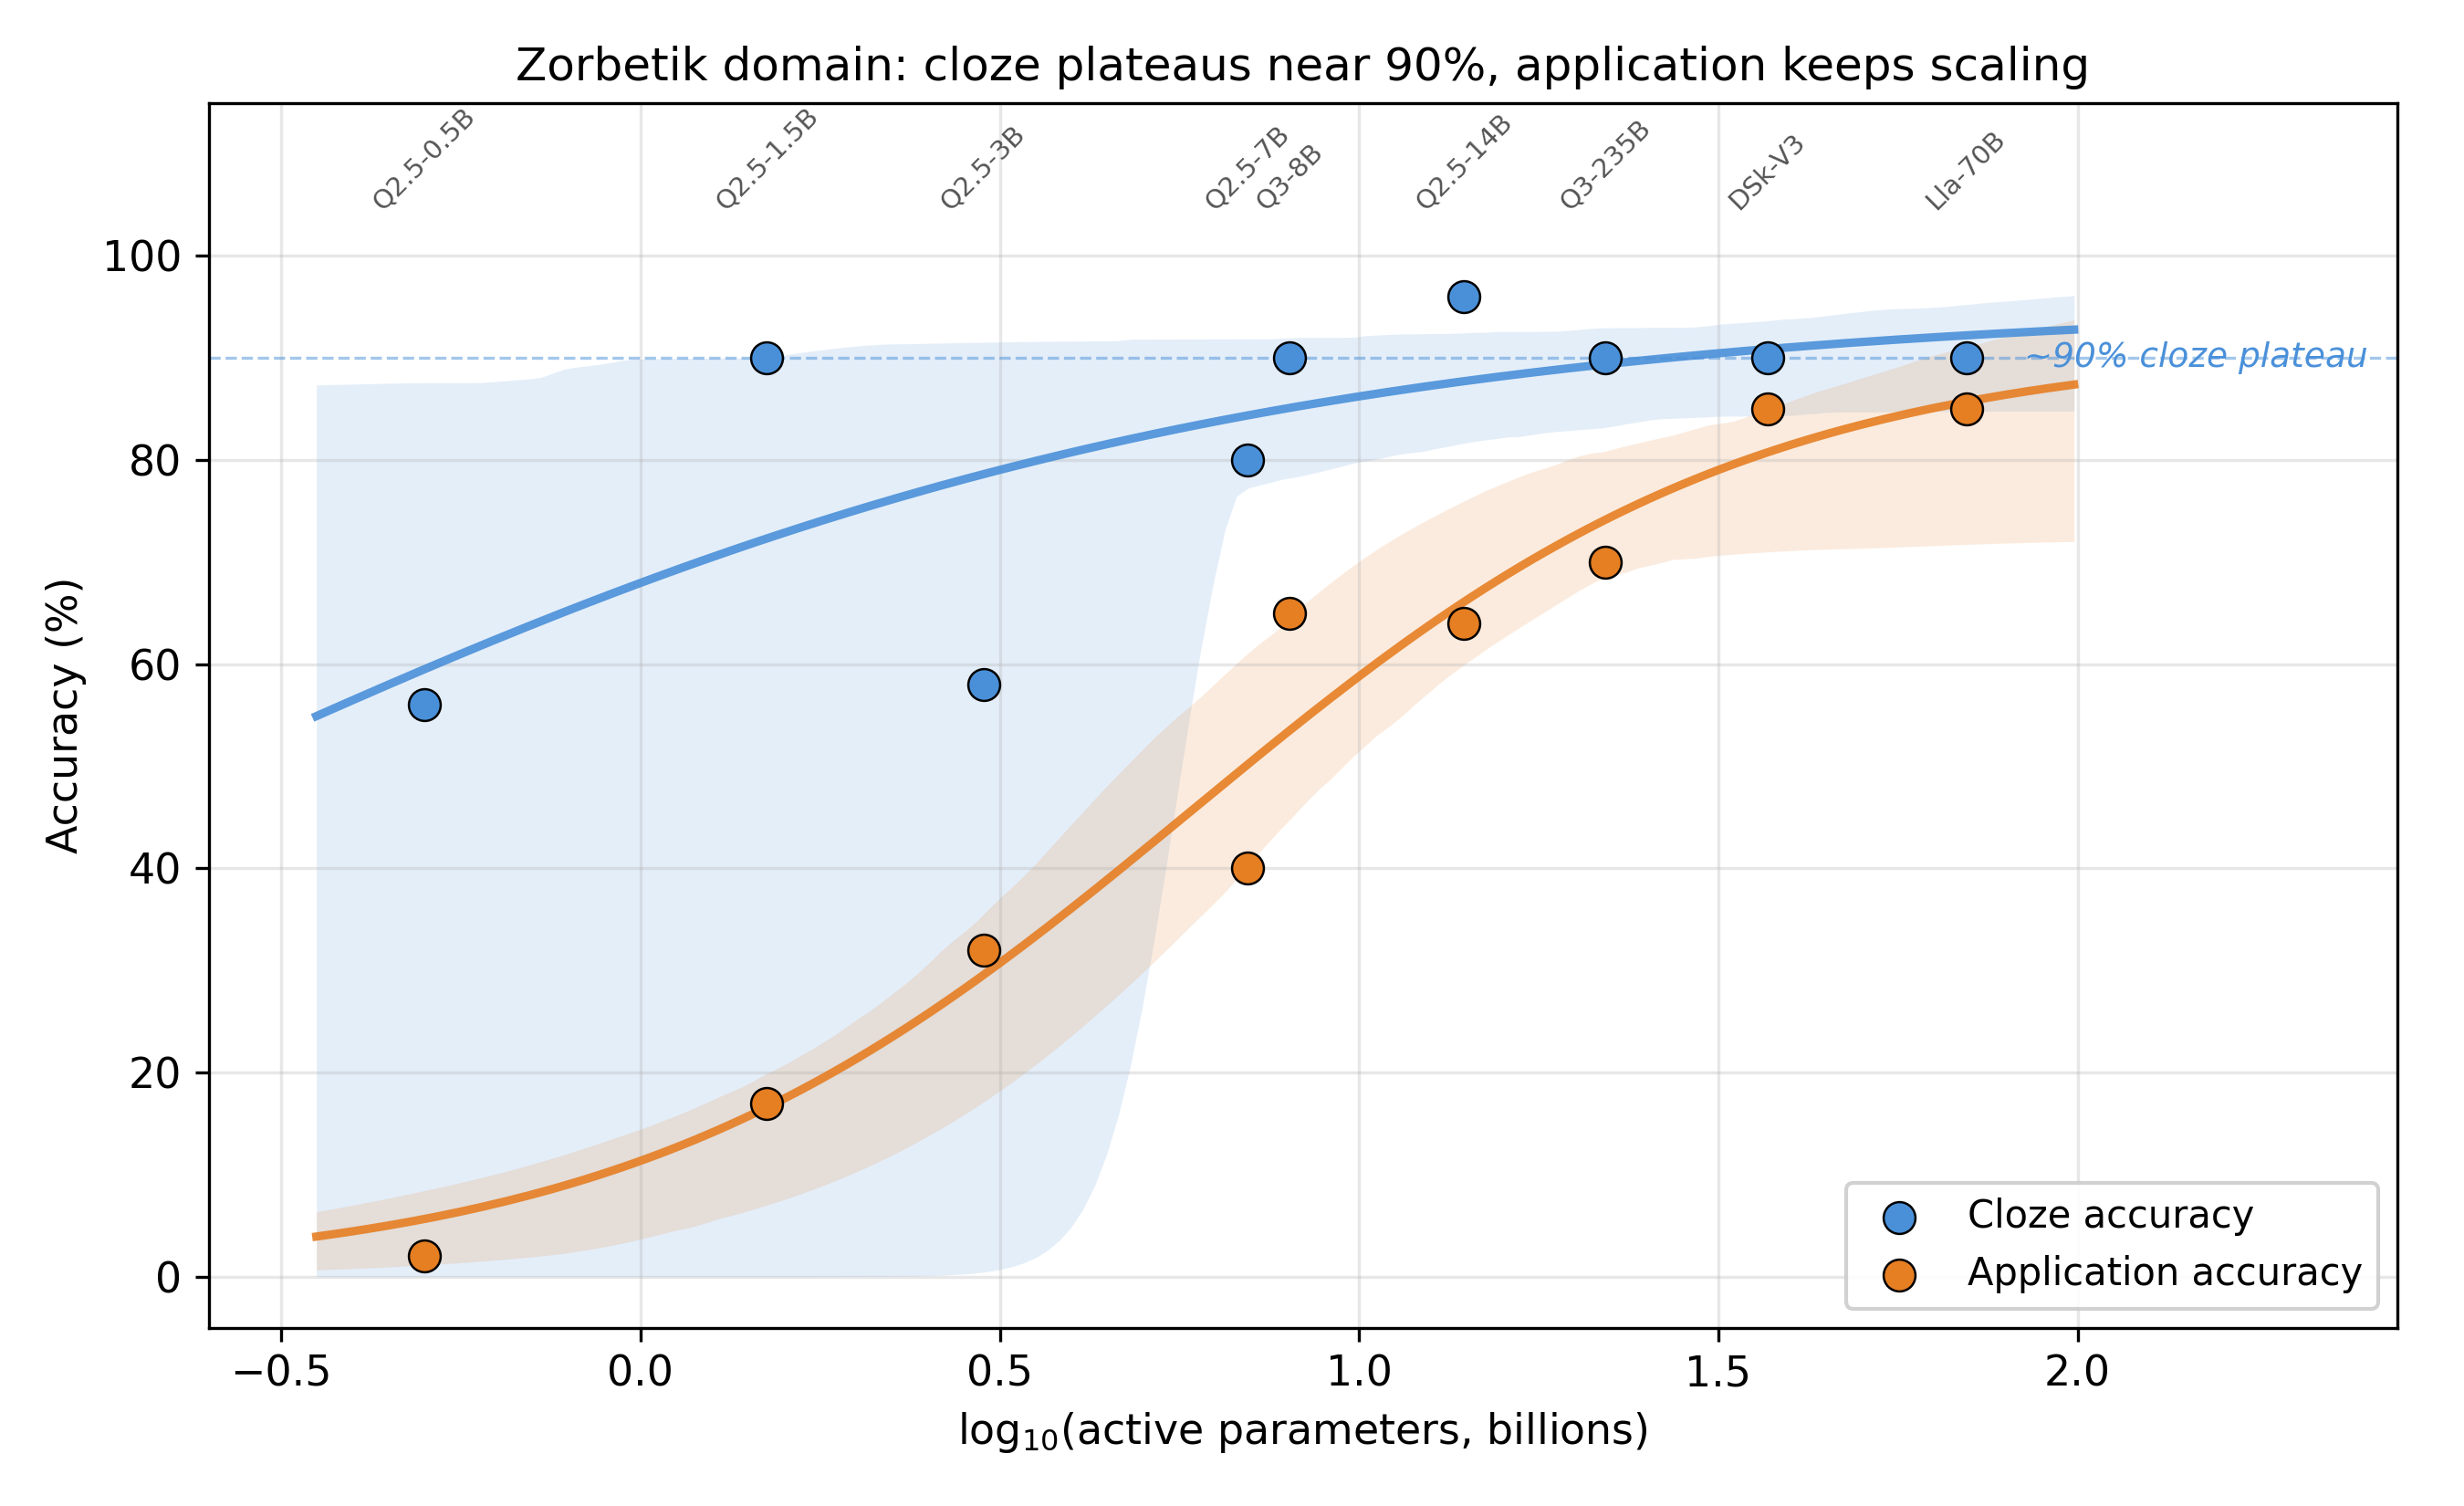
\includegraphics[keepaspectratio,alt={Figure 1: Capacity scaling on Zorbetik}]{figures/fig1_capacity_scaling.png}}
\caption{Figure 1: Capacity scaling on Zorbetik}
\end{figure}

\textbf{Figure 1.} Cloze (blue) and application (orange) accuracy as a
function of log₁₀(model size in billions of active parameters) across
nine models. Points show the observed accuracy; shaded bands show 95\%
bootstrap confidence intervals around a logistic fit. Cloze saturates at
\textasciitilde90\% by 8B parameters. Application scales monotonically
across three orders of magnitude, reaching 85\% at 70B active
parameters. The gap between the two curves operationalises
``intelligence headroom'' on this domain --- how much further capacity
can carry the model before application saturates too.

\begin{figure}
\centering
\pandocbounded{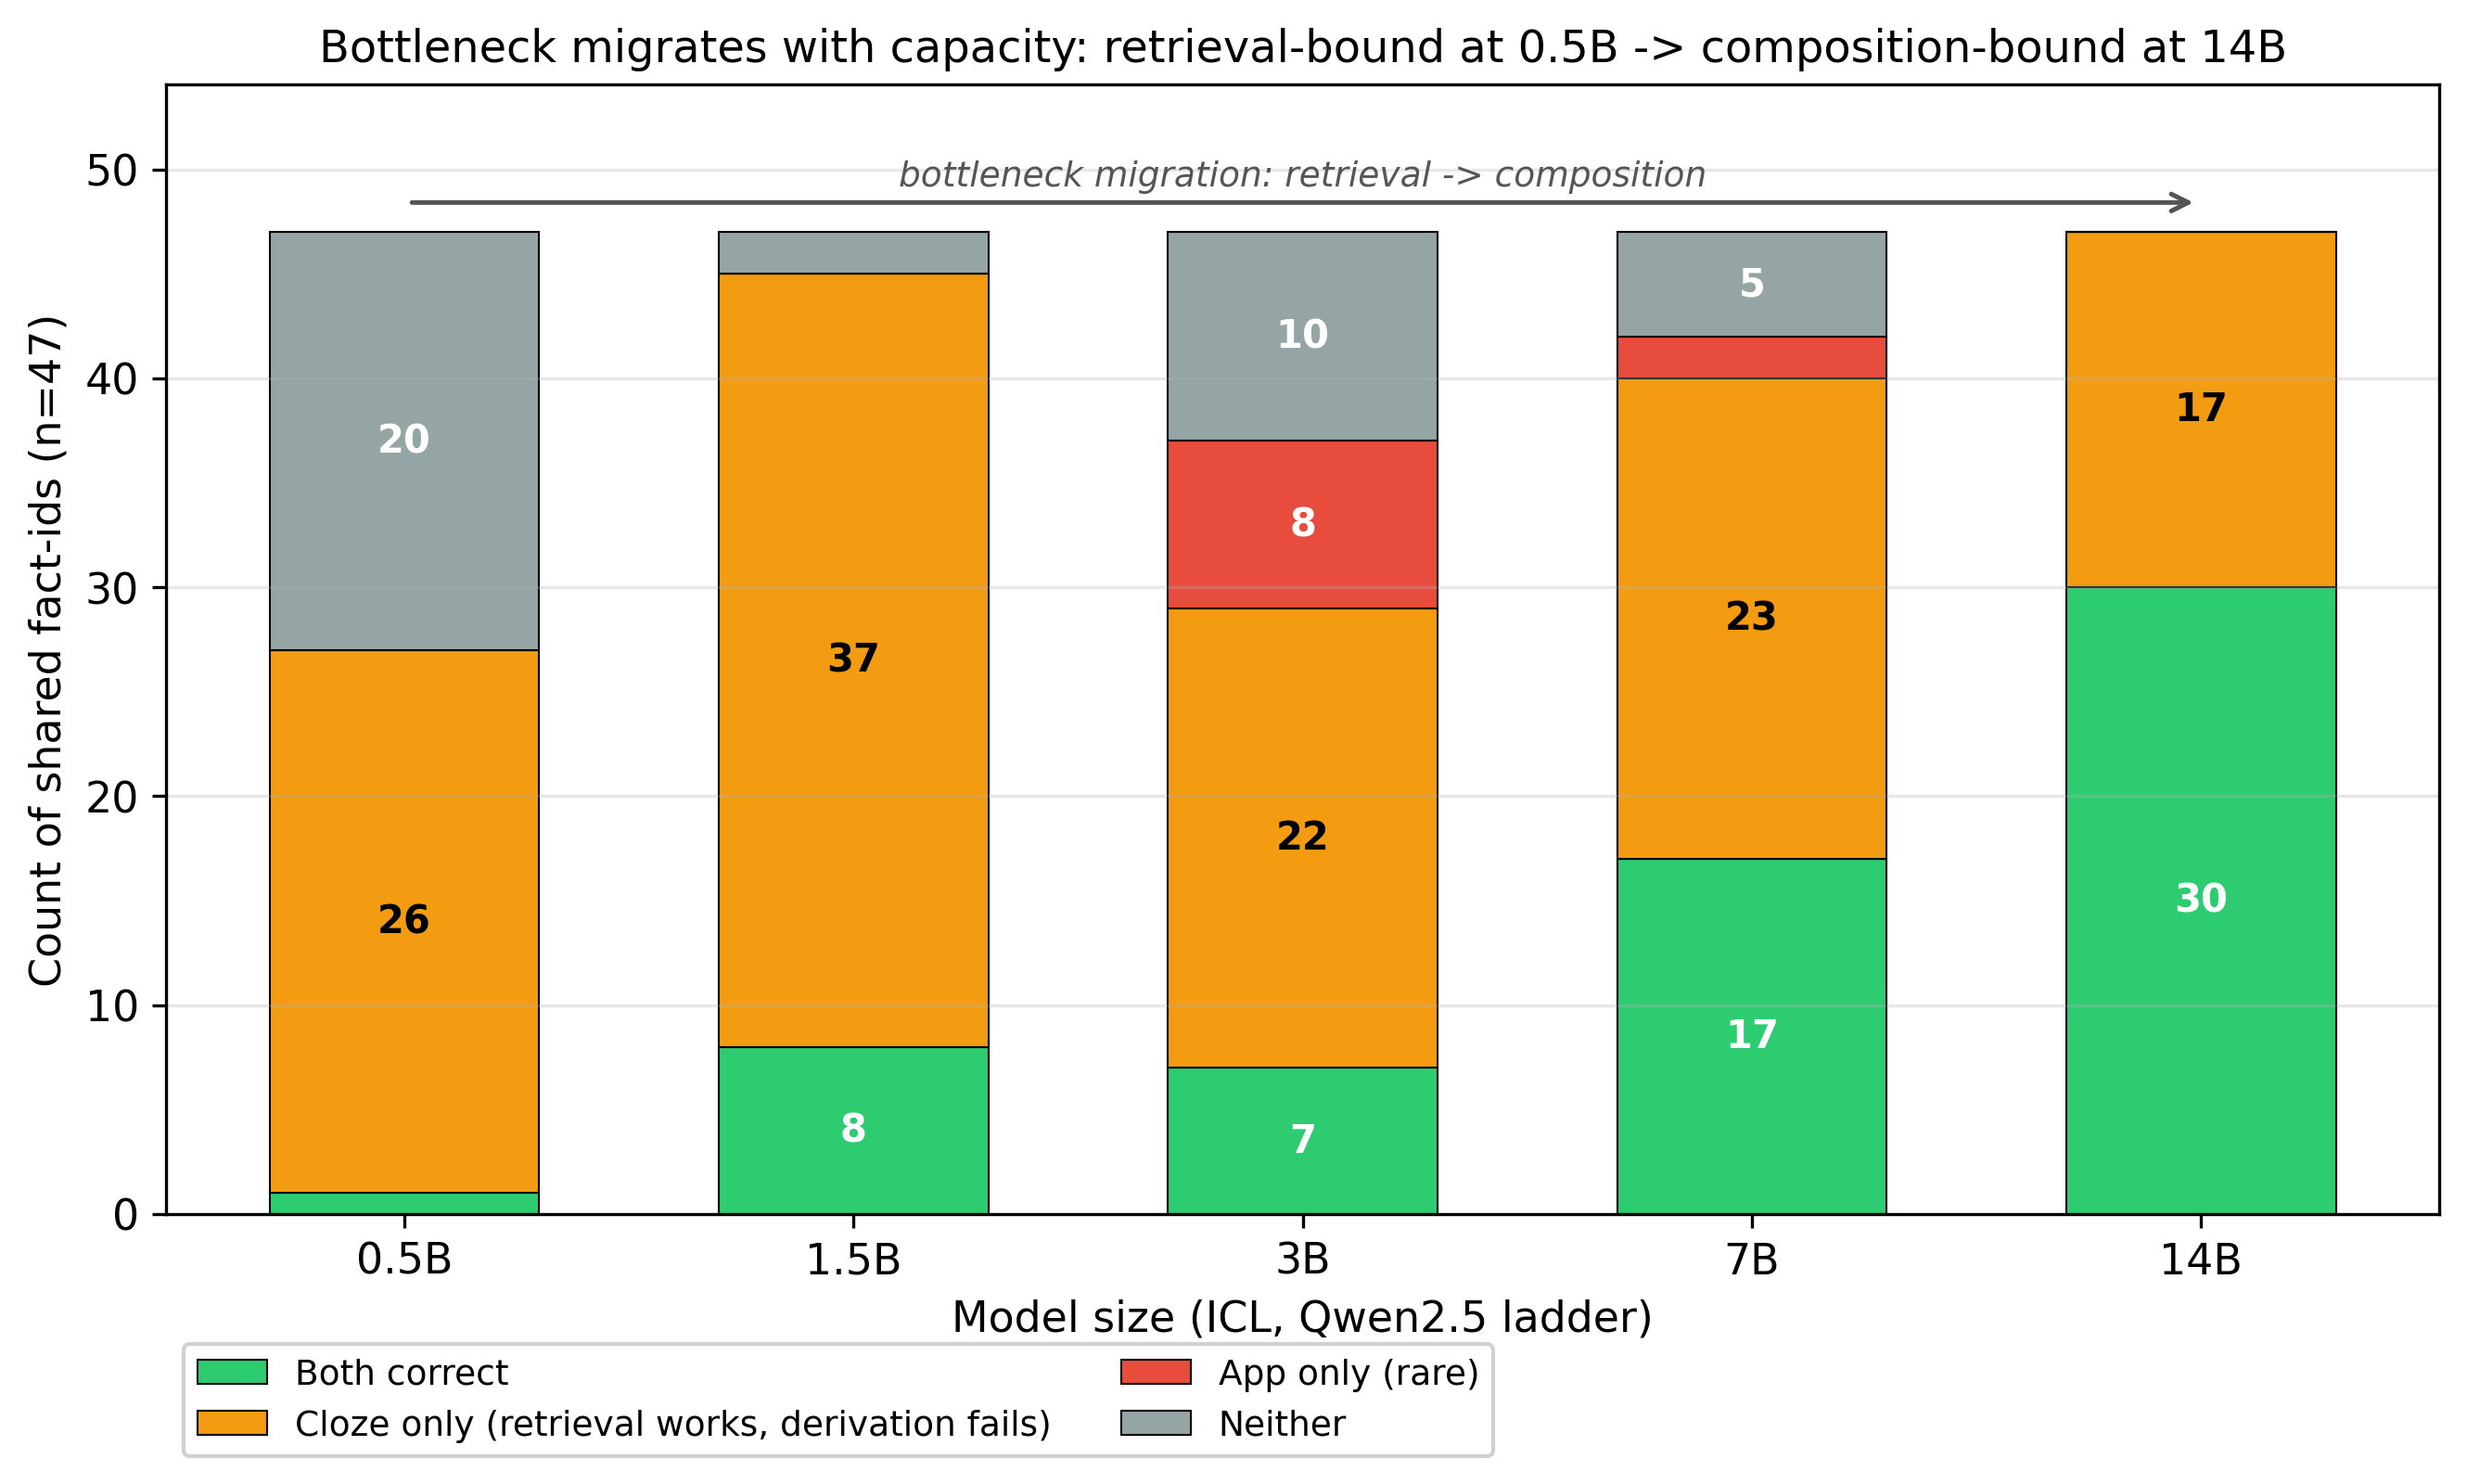
\includegraphics[keepaspectratio,alt={Figure 2: Bottleneck migration across capacity}]{figures/fig2_bottleneck_migration.png}}
\caption{Figure 2: Bottleneck migration across capacity}
\end{figure}

\textbf{Figure 2.} Per-fact-id outcome composition across five model
sizes on the 47 facts that appear in both cloze and application banks.
At 0.5B, the dominant failure mode is retrieval (``Neither'' + small
``App-only'' bars); by 7-14B, retrieval is essentially saturated and the
remaining failure is composition-bound (``Cloze-only'': 17/47 = 36\% at
14B). The bottleneck \emph{location} shifts with capacity --- precisely
what the C-axis prediction implies.

\begin{figure}
\centering
\pandocbounded{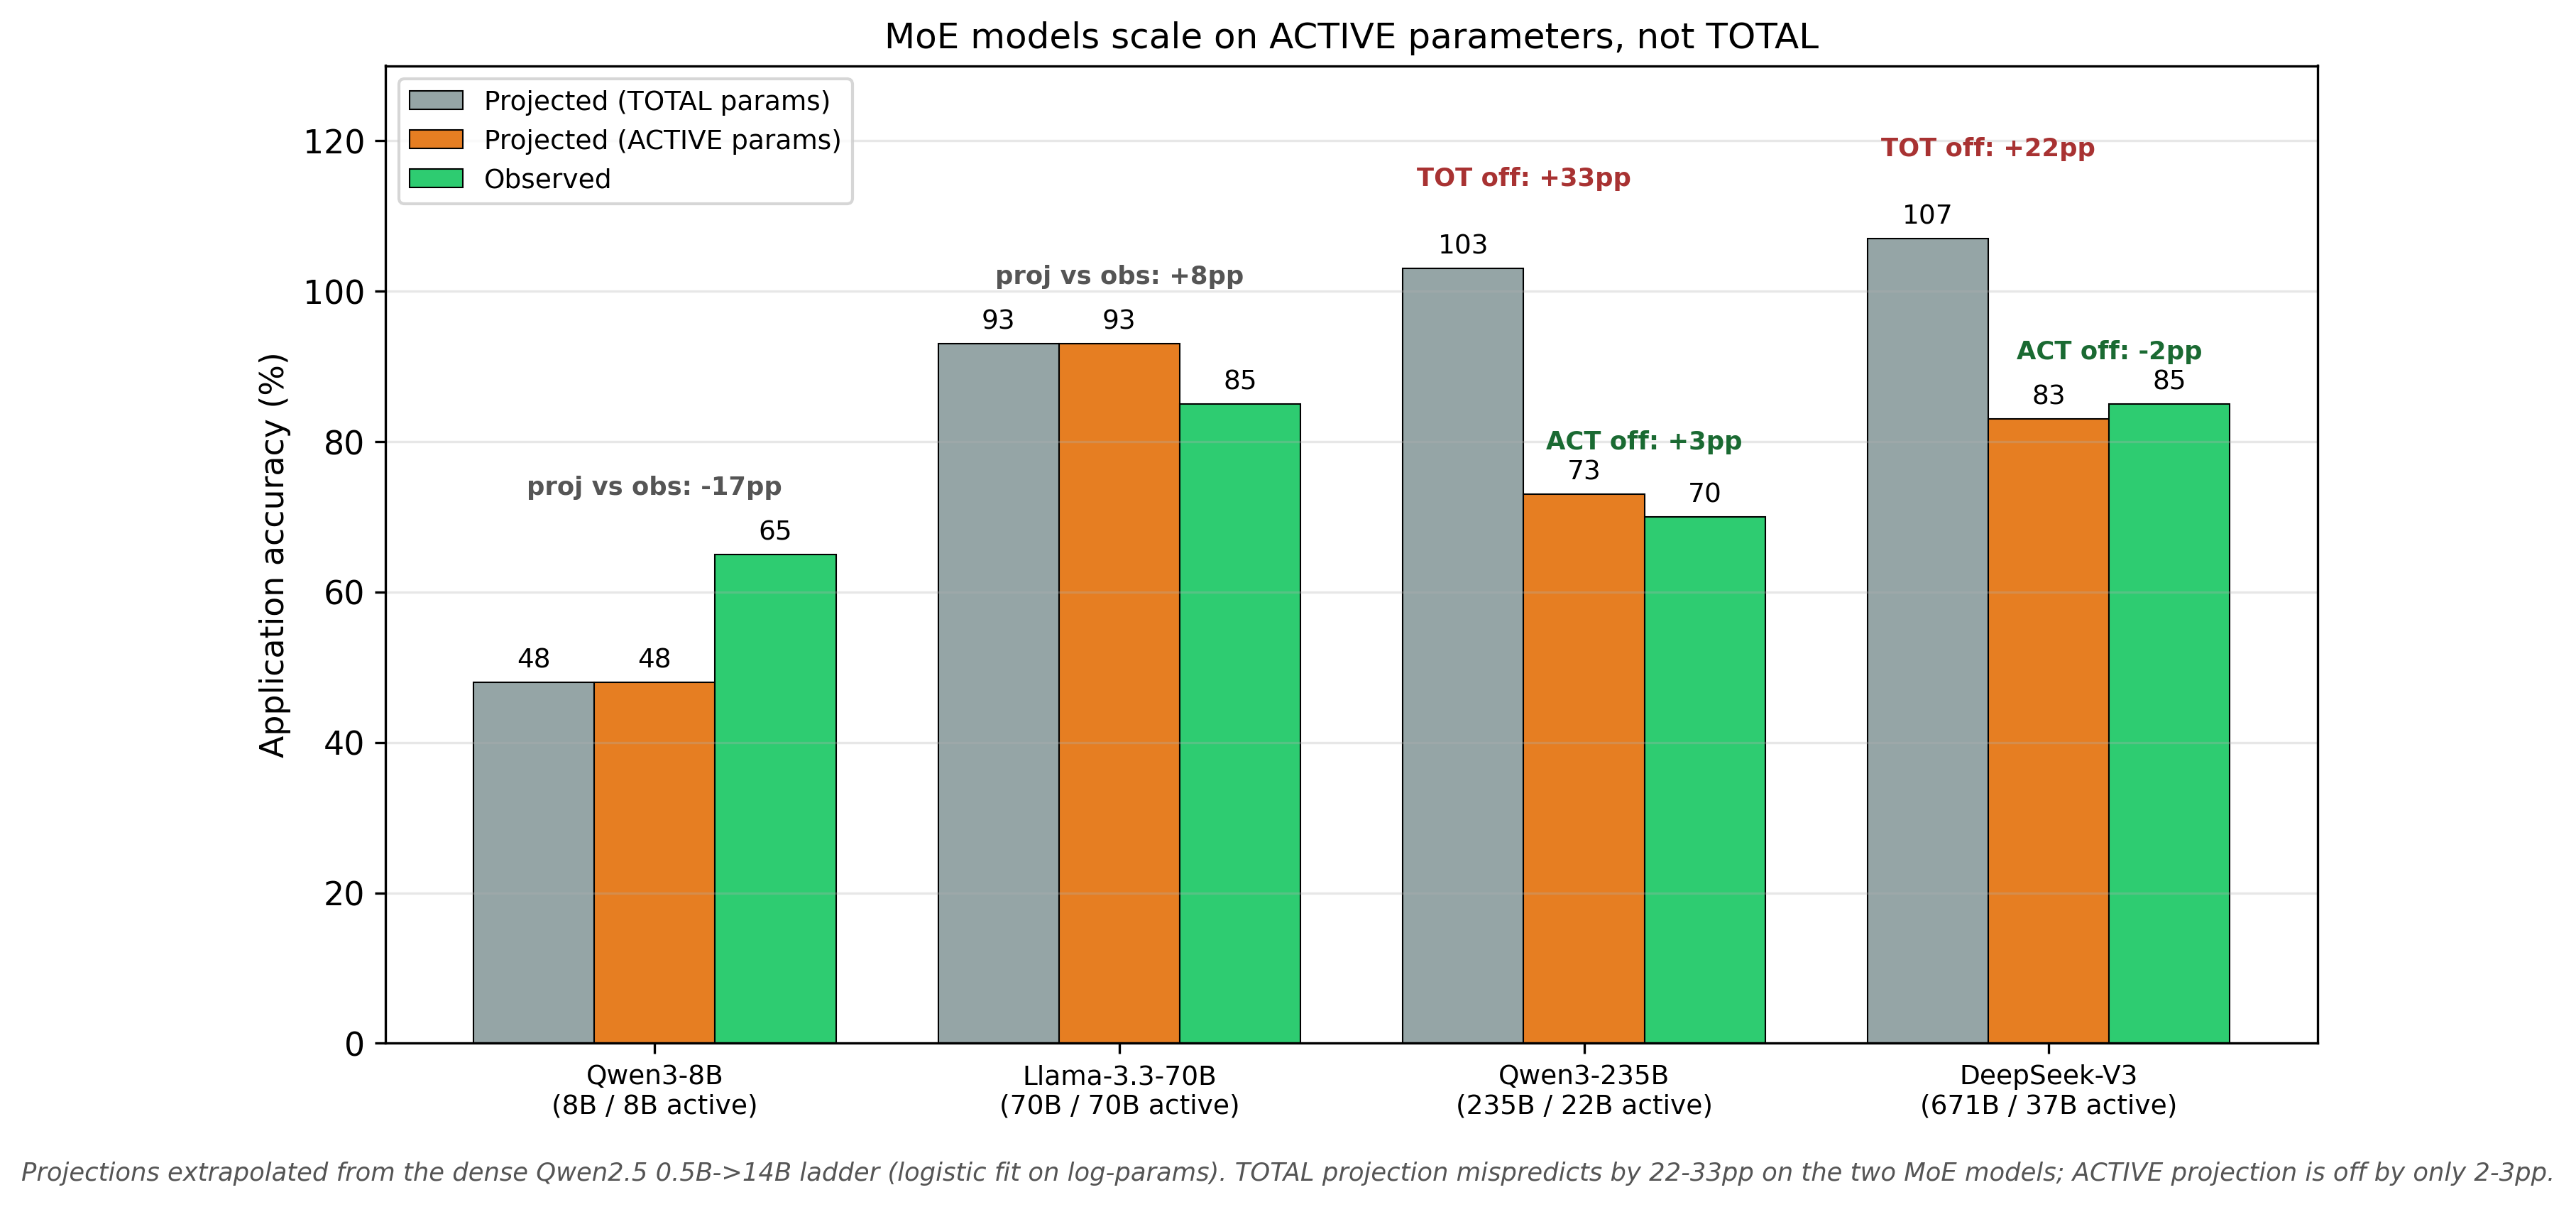
\includegraphics[keepaspectratio,alt={Figure 3: MoE active vs total parameter projection}]{figures/fig3_moe_active_vs_total.png}}
\caption{Figure 3: MoE active vs total parameter projection}
\end{figure}

\textbf{Figure 3.} Logistic-fit projections (from the dense Qwen2.5
0.5B→14B sub-ladder) applied to four large-model anchors, using either
TOTAL parameters (light bars) or ACTIVE parameters (darker bars),
compared against the actually observed accuracy (dashed line). For dense
models (Qwen3-8B, Llama-3.3-70B) TOTAL and ACTIVE are identical. For the
two MoE models (Qwen3-235B at 22B active, DeepSeek-V3 at 37B active),
the ACTIVE-parameter projection lands within 3pp of the observation
while the TOTAL-parameter projection is off by 22-33pp. Effective
compute capacity is determined by per-token active parameters, not by
total parameter count.

\subsubsection{Table 1 --- Per-model
summary}\label{table-1-per-model-summary}

Per-model cloze and application accuracy, plus per-token CR statistics
(median, first-5, last-5) computed over application responses. See
\href{tables/table1_per_model_summary.md}{\texttt{tables/table1\_per\_model\_summary.md}}
for the full table with platform-dependency footnotes.

{\def\LTcaptype{none} % do not increment counter
\begin{longtable}[]{@{}lrrrrr@{}}
\toprule\noalign{}
Model & Size (B) & Active (B) & Cloze \% & Application \% & n\_resp \\
\midrule\noalign{}
\endhead
\bottomrule\noalign{}
\endlastfoot
Qwen2.5-0.5B & 0.5 & 0.5 & 56 & 2 & 47 \\
Qwen2.5-1.5B & 1.5 & 1.5 & 90 & 17 & 47 \\
Qwen2.5-3B & 3 & 3 & 58 & 32 & 47 \\
Qwen2.5-7B & 7 & 7 & 80 & 40 & 47 \\
Qwen3-8B & 8 & 8 & 90 & 65 & 20 \\
Qwen2.5-14B & 14 & 14 & 96 & 64 & 47 \\
Llama-3.3-70B & 70 & 70 & 90 & 85 & 20 \\
Qwen3-235B & 235 & 22 & 90 & 70 & 20 \\
DeepSeek-V3 & 671 & 37 & 90 & 85 & 20 \\
\end{longtable}
}

CR statistics are reported in the full table linked above; they span
multiple orders of magnitude because the hosted-API platforms
(Fireworks, Together) return logprobs clipped to ≈−10⁻⁵ on confident
tokens, inflating the CR denominator. Within-platform CR comparisons are
valid; cross-platform absolute comparisons are not. On the Qwen2.5
ladder (locally served, uniform platform), last5\_cr systematically
exceeds first5\_cr from 3B upward --- consistent with the §2.8
observation that application friction accumulates during the reasoning
chain rather than spiking on the first token.

\begin{center}\rule{0.5\linewidth}{0.5pt}\end{center}

\subsection{8. References}\label{references}

Akyürek, E., Schuurmans, D., Andreas, J., Ma, T. \& Zhou, D. (2022).
What learning algorithm is in-context learning? \emph{arXiv:2211.15661}.

Brown, T. B., Mann, B., Ryder, N. et al.~(2020). Language models are
few-shot learners. \emph{NeurIPS 2020}. arXiv:2005.14165.

Craik, F. I. M. \& Lockhart, R. S. (1972). Levels of processing: a
framework for memory research. \emph{Journal of Verbal Learning and
Verbal Behavior}, 11, 671--684.

Dai, D., Sun, Y., Dong, L., Hao, Y., Sui, Z. \& Wei, F. (2022). Why can
GPT learn in-context? \emph{arXiv:2212.10559}.

Damásio, A. (1994). \emph{Descartes' Error: Emotion, Reason, and the
Human Brain}. Putnam.

Geva, M., Schuster, R., Berant, J. \& Levy, O. (2021). Transformer
feed-forward layers are key-value memories. \emph{EMNLP 2021}.
arXiv:2012.14913.

Gudibande, A., Wallace, E., Snell, C., Geng, X., Liu, H., Abbeel, P.,
Levine, S. \& Song, D. (2023). The false promise of imitating
proprietary LLMs. \emph{arXiv:2305.15717}.

Kalyuga, S., Ayres, P., Chandler, P. \& Sweller, J. (2003). The
expertise reversal effect. \emph{Educational Psychologist}, 38, 23--31.

Lund, T. (2026a). Behavioural Friction Theory: A race-based account of
decision cost in human cognition. Zenodo preprint. DOI:
10.5281/zenodo.19462500.

Lund, T. (2026b). Friction as the cost of probabilistic computation: A
generalised substrate theory. Target: \emph{Behavioural and Brain
Sciences}. {[}Paper 1, this series.{]}

Lund, T. (2026d). Friction-guided inference: a free signal that improves
any LLM. {[}Paper 3, this series, in preparation.{]}

Lund, T. (2026e). Cross-substrate replication of classical learning
phenomena on LLM substrate. {[}Paper 4, this series, in preparation.{]}

Lund, T. (2026f). A recursive strategy-choice race account of expertise
reversal. {[}Paper 4B, this series, in preparation.{]}

Lund, T. (2026h). Matched friction under hysteresis: A unifying
principle for learning optima. {[}Paper 6, this series, in
preparation.{]}

McClelland, J. L., McNaughton, B. L. \& O'Reilly, R. C. (1995). Why
there are complementary learning systems in the hippocampus and
neocortex. \emph{Psychological Review}, 102, 419--457.

Paivio, A. (1971). \emph{Imagery and Verbal Processes}. Holt, Rinehart
\& Winston.

Schaeffer, R., Miranda, B. \& Koyejo, S. (2023). Are emergent abilities
of large language models a mirage? \emph{NeurIPS 2023}.
arXiv:2304.15004.

Soudani, H., Kanoulas, E. \& Hasibi, F. (2024). Fine tuning
vs.~retrieval augmented generation for less popular knowledge.
\emph{arXiv:2403.01432}.

Yonelinas, A. P., Ranganath, C., Ekstrom, A. D. \& Wiltgen, B. J.
(2019). A contextual binding theory of episodic memory: systems
consolidation reconsidered. \emph{Nature Reviews Neuroscience}, 20(6),
364--375. DOI: 10.1038/s41583-019-0150-4.

\end{document}
